\section[Построение кривых Безье. Иллюстрация хода построения]{Построение кривых Безье. Иллюстрация хода построения}
Используя инструмент \textit{\textbf{Beezierline}}, строим кривые, данные в тексте работы.

Построение кривых иллюстрируем опорными линиями (инструмент \textit{\textbf{Line}}):
\hspace{0pt}
\begin{figure}[H]
    \begin{minipage}[h]{0.333\linewidth}
        \center{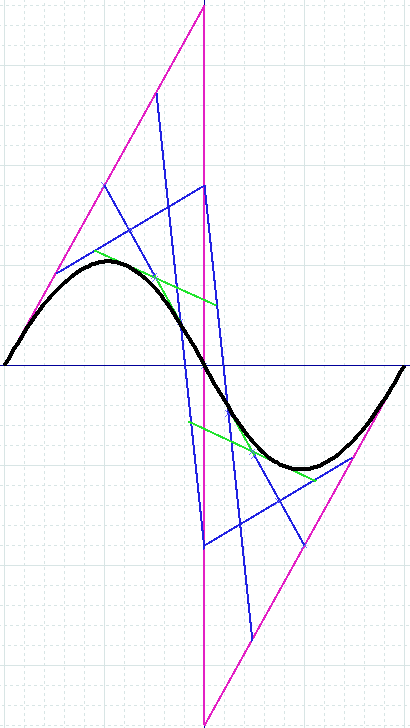
\includegraphics[width=1\linewidth]{1_1_sin.png}} (одна кривая Безье) \\
    \end{minipage}
    \hfill
    \begin{minipage}[h]{0.47\linewidth}
        \center{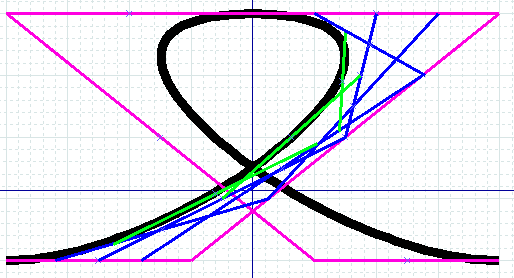
\includegraphics[width=1\linewidth]{1_3_loop.png}} \\(две кривые Безье)
    \end{minipage}
    \hfill
    \center
    \begin{minipage}[h]{0.9\linewidth}
        \center{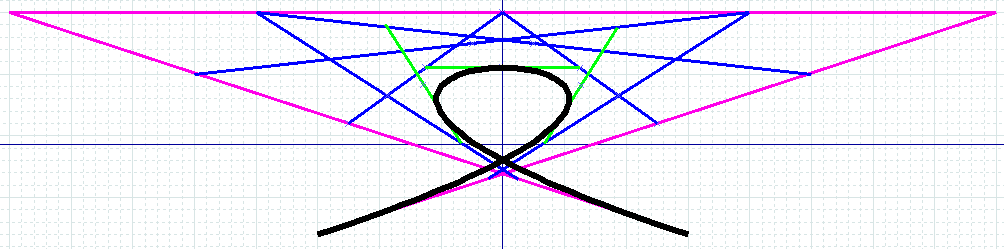
\includegraphics[width=1\linewidth]{1_2_loop.png}} (одна кривая Безье) \\
    \end{minipage}
\end{figure}

Опорные линии первого уровня -- \textbf{\textit{зеленый}}, 
второго уровня -- \textbf{\textit{синий}}, 
третьего уровня -- \textbf{\textit{розовый}}.
